%   Filename    : chapter_4.tex 
\chapter{Research Methodology}

\section{Description and Functionality of TESS}
TESS is a computerized reading assessment program that will allow students to take the SORT with minimal to no assistance from a teacher. The following steps described were specifically requested and specified by the faculty-in-charge of ICNHS' reading remediation program.

In this computerized SORT, students will read out loud from a randomized list of words flashed to them, word-by-word on the screen. This list of words is predetermined and is categorized by reading level. If the student is deemed correct, the program will proceed with the next word in the list. If the student was incorrect, then the program will remain at the current word. The student is allowed to attempt the word three times, with a timer of 10 seconds per attempt.

Additionally, the faculty wants to decrease the amount of stress and frustration the examinee will experience during the assessment, so TESS includes a built-in timer for each item in the test. Once eleven (11) seconds have passed an item will be skipped, and once ten words in a row have been skipped, the test will end and the examinee’s reading level will be calculated.

A progress bar will also be visible in the bottom, so that students are able to track their progress through the assessment.

The program will also evaluate the students and provide the teacher with an excel sheet for each student containing their results, which includes an itemized list of which words in the SORT they got right and wrong.

The test portion of the program is voice activated, and the examinee can make use of certain keywords to navigate through the test. Such as START to start the test; SKIP to skip a word; and STOP to end the test prematurely.

TESS should be able to run on an offline computer with a headset.

\subsection{Voice Functionality and Collected Voice Data}
TESS’ voice functionality is the most important part of the program. The speech-to-text program included should be able to function in a school environment and also be able to accurately assess accented English.

Student’s voice will be recorded by the program, assessed, and then discarded. The program does not need to store data of any examinee’s voice to function.

\subsubsection{Other Collected Data}
TESS will take note of the following information:
\begin{itemize}
\item Student Name
\item Student’s School
\item Proctor’s Name
\end{itemize}
This information is used to generate the excel report after the test is finished. TESS does not save this data after the completion of the test.

\section{Developing TESS}
TESS is developed using Python and a voice recognition software.
The three main choices for our voice recognition software are the following:
\begin{itemize}
\item Vosk,
\item Wav2Vec, and
\item Whisper
\end{itemize}
These software were chosen because all three are open source software and do not require any payment to keep it running.
The program is also designed to work on a computer with a dedicated headset and microphone.

In order to determine which of the three to use, we developed a TESS prototype that can evaluate the voice input using all three software. We then conducted an informal test to see which of the three is most effective.

However, Whisper was out of the running early on as it was unable to be run quickly enough to use in real time. This left Vosk and Wav2Vec to be tested.

After further research we decided to use Vosk. Vosk was chosen because of the following advantages:
\begin{enumerate}
\item Offline Capability,
\item Lightweight and Fast,
\item Customizable Models,
\item Open-Source, and 
\item Cost-Effective.
\end{enumerate}

Although, Vosk does have a few disadvantages. Most notably, it has difficulty dealing with the following:
\begin{enumerate}
    \item Accuracy with Complex Speech,
    \item Limited Support for Certain Accents, or Dialects
    \item Limited Context Understanding.
\end{enumerate}

In order to further improve Vosk’s accuracy in dealing with complex speech as well as to deal with accented English, Jellyfish was used in the post-processing. Jellyfish compares two strings to see how phonetically close they are.

The program is also designed to work on a computer with a dedicated headset and microphone.

{\clearpage}
\section{GUI Mockup}
The following are images of the current GUI of Tess.

\begin{figure}[h]
   \centering
   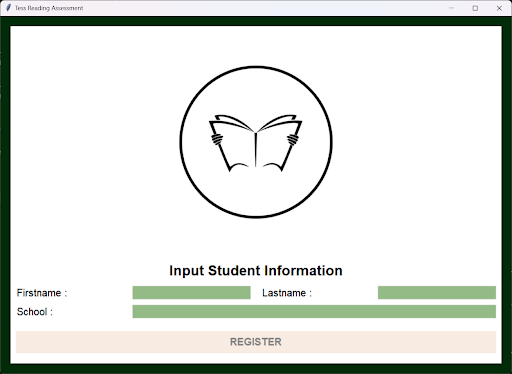
\includegraphics[scale = 0.6]{figures/Student-Input-Screen.png}
   \caption{Student Input Screen.}
    \label{fig:studentInput}
\end{figure}

\begin{figure}[!]
   \centering
   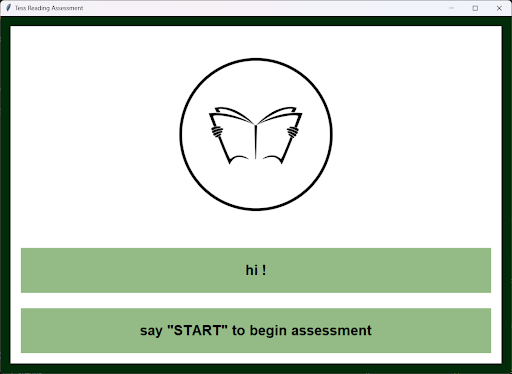
\includegraphics[scale = 0.6]{figures/Pre-test-Screen.png}
   \caption{Pre-test Screen.}
    \label{fig:pretestScreen}
\end{figure}

\begin{figure}[!]
   \centering
   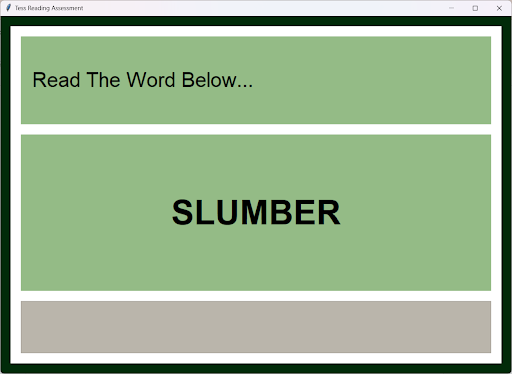
\includegraphics[scale = 0.6]{figures/Test-Screen.png}
   \caption{Test Screen.}
    \label{fig:testScreen}
\end{figure}

\begin{figure}[!]
   \centering
   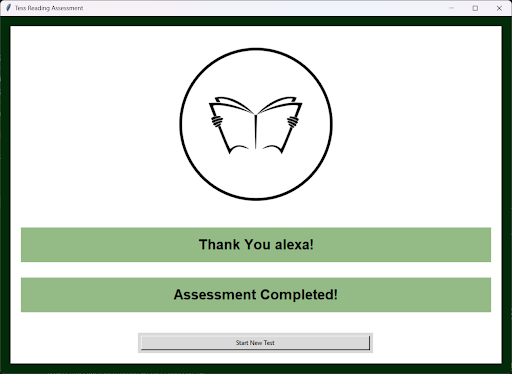
\includegraphics[scale = 0.6]{figures/Post-test-Screen.png}
   \caption{Post-test Screen.}
    \label{fig:posttestScreen}
\end{figure}

{\clearpage}

\section{Testing the Program}
TESS will be tested at the Iloilo City National High School with a group of ten (10) random Grade 7 students.

The group will take the manual SORT and the computerized SORT through TESS at the same time -- this is to avoid practice bias. The testing duration will be timed, and the results of the tests will be used to determine the efficacy of TESS in relation to a manual SORT.

After the testing, a focus group discussion will be held to determine what the user experience was like.

TESS will then be compared with Manual SORT along the following metrics:
\begin{itemize}
\item Speed - how fast does each student complete their assessment?
\item Accuracy - how accurate are the results of each student?
\item Ease of Use - how easy was the test to be administered / taken?
\end{itemize}

The Speed and Accuracy metrics can be determined using the information gathered during the assessment. However, the Ease of Use metric will be derived from a Focus Group Discussion composed of participating students and faculty.

\subsection{Software Evaluation Form}
To evaluate how effective TESS is along the Speed, Accuracy, and Ease of Use metrics, we have created an evaluation form.

While the main categories are Speed, Accuracy, and Ease of Use, they will be further expanded into relevant questions which will allow the researchers to better gauge TESS’ performance in each of those metrics.
{\clearpage}
For each metric and its corresponding descriptive characteristic, TESS will be graded on a scale of 1 to 5; with 1 being “Poor” and 5 being “Very Good”. The scale is as follows, from least to greatest.
\begin{enumerate}
    \item Poor (P)
    \item Fair (F)
    \item Average (A)
    \item Good (G)
    \item Very Good (VG)
\end{enumerate}

\begin{figure}[h]
   \centering
   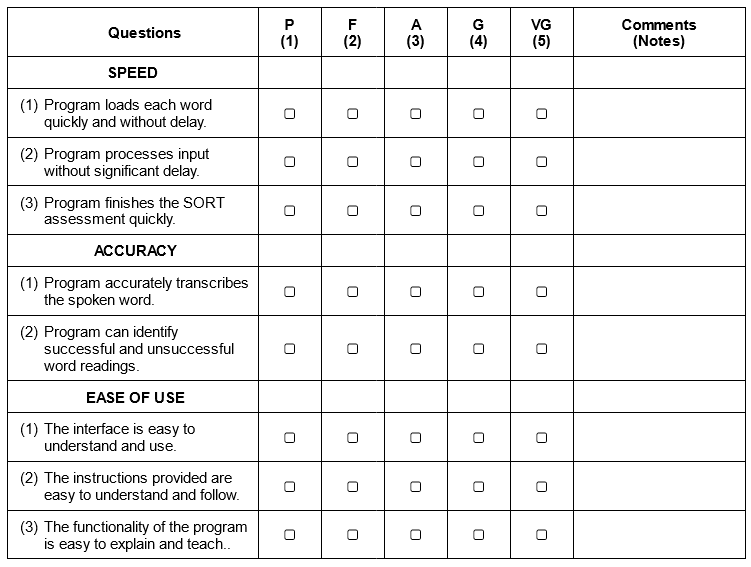
\includegraphics[scale=0.6]{figures/TESS-software-eval.png}
   \caption{Software Evaluation Form.}
    \label{fig:softwareEval}
\end{figure}


\subsection{Focus Group Discussion Outline}
The focus group discussion will center around the experience of the faculty and students while using TESS. The discussion will last for around 30 minutes. The following is the set of questions we will use as a guideline for the discussion. 

\begin{enumerate}
\item What was the experience of using TESS to take the reading test like?
\item How did using TESS differ from taking / administering SORT manually?
\item What difficulties did you encounter while using TESS?
\item Among the TESS models, which one did you like using most?
\item If you could add one feature or function to TESS what would it be?
\end{enumerate}

\subsection{Consent Forms}
\subsection{Consent Forms}
Students participating in the TESS testing will be required to fill out parental consent forms in order to participate.
There are two forms. One in English, and one in Hiligaynon.
